% *******************************************************************************
% * Copyright (c) 2007 by Elexis
% * All rights reserved. This document and the accompanying materials
% * are made available under the terms of the Eclipse Public License v1.0
% * which accompanies this distribution, and is available at
% * http://www.eclipse.org/legal/epl-v10.html
% *
% * Contributors:
% *    G. Weirich - initial implementation
% *
% *  $Id: rest.tex 2933 2007-07-29 10:05:35Z rgw_ch $
% *******************************************************************************
% !Mode:: "TeX:UTF-8" (encoding info for WinEdt)

\section{Diverse Views}

\subsection{Datenanzeige}
Dies ist eine View, die beliebige Felder der Elexis-Datenbank anzeigen
kann. Mehrere Exemplare dieser View können (mit unterschiedlichen oder denselben
Inhalten) in einer Perspektive eingebunden werden (S. Abb. \ref{figure1}).
\begin{figure}[hb]
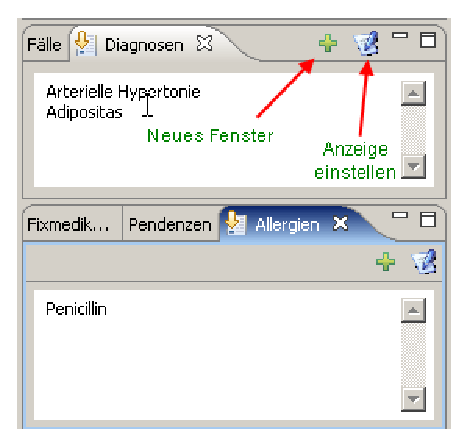
\includegraphics{images/data1}
\caption{Zwei Fenster der 'Datenanzeige'}
\label {figure1}
\end{figure}
Durch Klick auf den \textbf{+} - Button können Sie ein weiteres Exemplar der
View öffnen, durch Druck auf den Editieren-Button können Sie die anzuzeigenden
Daten einstellen.

\begin{figure}[hb]
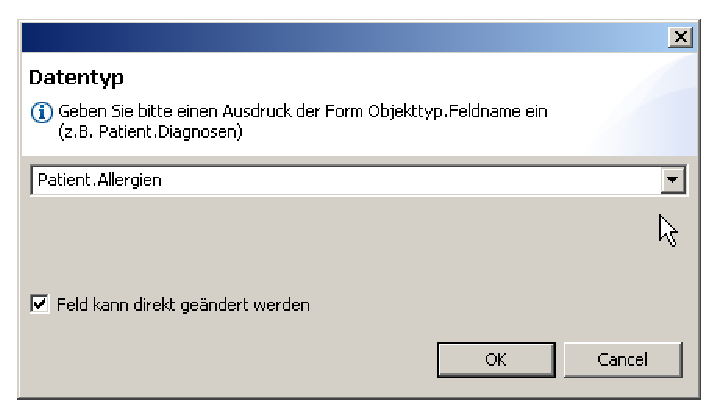
\includegraphics{images/data2}
\caption{Eingabedialog für den Datentyp}
\label{figure2}
\end{figure}
Es erscheint dann eine Dialogbox wie in Abb. \ref{figure2}.
Sie können hier jeden Datentyp einsetzen, der auch in Textvorlagen als
Platzhalter verwendet werden kann (Vgl. S. \pageref{Platzhalter}).
Wenn Sie die Checkbox 'Feld kann geändert werden' ankreuzen, dann können die
Daten (ausreichende Rechte vorausgesetzt) direkt durch Schreiben in dieses
Fenster geändert werden.
Die Anordnung und der Inhalt der Datenanzeige-Views werden beim Verlassen von
Elexis, oder bei Betätigen der Menüaktion 'Perspektive speichern' gespeichert.

\subsection{Fixmedikation}
Diese View zeigt die Fix- oder Dauermedikation des aktuell selektierten
Patienten an (S. Abb. \ref{fig:fixmedi})

\begin{figure}[htp]
\begin{center}
  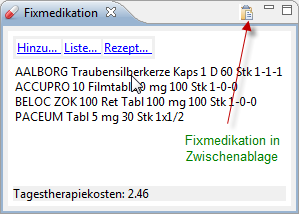
\includegraphics{images/fixmediview}
  \caption{Fixmedikation}
  \label{fig:fixmedi}
\end{center}
\end{figure}
Sie können Medikamente aus dem Artikel-Fenster oder aus einem Rezept in diese
View ziehen, und Sie können auch Artikel aus der Fixmedikation in ein Rezept
ziehen. Mit Klick auf \glqq Hinzu\ldots\grqq{} öffnen Sie die Artikel-View. Mit
Klick auf \glqq Liste\ldots\grqq{} erstellen Sie eine Einnahmeliste für den
Patienten. Dazu muss eine Textvorlage namens \glqq Einnahmeliste\grqq{}
existieren, und diese muss an einer Stelle den Platzhalter [Medikamentenliste]
enthalten. Mit Klick auf \glqq Rezept\grqq{} erstellen Sie ein Rezept mit der
Dauermedikation. Hierzu muss eine Textvorlage namens \glqq Rezept\grqq
existieren, welche an einer Stelle den Platzhalter [Rezeptzeilen] enthält.

\subsection{Medikamenten-Verlauf}
Diese View zeigt alle Medikamente, die beim aktuellen Patienten je verschrieben oder abgegeben worden sind, mit Datum und Dosierung (falls angegeben). Durch Klick auf die entsprechenden Spaltenköpfe können Sie nac Abgabedatum oder Medinamen sortieren. Bei Medikamenten aus der Fixmedikation wird ausserdem, falls gegeben, das Stopdatum angezeigt.

\subsection{Kompendium online}
Wenn Sie eine aktive Internet-Verbindung haben, dann wird in dieser View das
Arzneimit\-tel-Kom\-pen\-dium der Schweiz angezeigt.

\subsection{Open Drug Database}
Diese View zeigt bei aktiver Internet-Verbindung die entsprechende Site an, die Sie z.. für die Suche nach Generika oder Interaktionen verwenden können.

\subsection{Pendenzen}
Erinnerungen, Reminders, Pendenzen: Diese View zeigt Ihnen Dinge an, an die Sie
denken mochten oder sollten (s. Abb. \ref{fig:pendenzen}).

\begin{wrapfigure}{l}{7.5cm}
  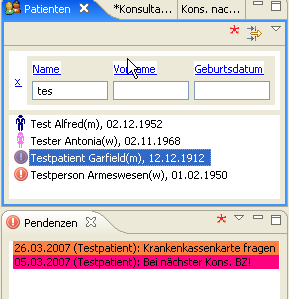
\includegraphics[width=7.2cm]{images/pendenzenview}
  \caption{Pendenzen-View}
  \label{fig:pendenzen}
\end{wrapfigure}

Eine Pendenz hat ein Fälligkeitsdatum und einen Status (geplant, fällig,
überfällig, erledigt, bleibt unerledigt).

Es gibt folgende Typen von Pendenzen:
\begin{itemize}
  \item Aufträge für eine bestimmte Person oder Aufträge an alle.
  \item Erinnerungen, die immer angezeigt werden, sobald ihr Fälligkeitsdatum
  erreicht oder überschritten ist.
  \item Erinnerungen, die nur dann angezeigt werden, wenn sie fällig sind
  \textit{und} wenn ein bestimmter Patient ausgewählt ist.
  \item Pendenzen, die nicht nur angezeigt werden, sondern die auch direkt eine
  bestimmte Aktion auslösen können (z.B. einen Serienbrief schreiben).
\end{itemize}

Wenn ein Patient fällige Pendenzen hat, dann wird in der Patientenliste das
Pendenzen-Symbol angezeigt (s. Abb. \ref{fig:pendenzen})

Um eine neue Pendenz zu erstellen, klicken Sie auf das Symbol \glqq Neue
Pendenz\grqq{}(roter Stern). Es erscheint dann eine Dialogbox, in der Sie Text,
typ, verantwortliche Person, Fälligkeitsdatum und anfänglichen Status der
Pendenz eingeben können.

Doppelklick auf eine Pendenz öffnet diese zum Bearbeiten. Es erscheint dieselbe
Dialogbox.

